\documentclass[12pt]{article}
\usepackage{graphicx}
\usepackage{caption}
\usepackage{subcaption}
\usepackage{siunitx}  
%
% Title.
\title{Experiment 2\\
Schmitt Trigger, Astable Multivibrator}

% Author
\author{Name of student,Roll. no.}

% begin the document.
\begin{document}

% make a title page.
\maketitle

\section{Overview of the experiment}
A Schmitt trigger is a comparator circuit with hysteresis implemented by applying positive feedback in an opamp. It is an active circuit which converts an analog input signal to a digital output signal.

An Astable Multivibrator or a Free Running Multivibrator is the multivibrator which has no stable states. Its output oscillates continuously between its two unstable states without the aid of external triggering.
\\
\\In this experiment we have realized both the above mentioned circuits using opamp IC741. The connections have been made on a breadboard and waveforms have been observed on a DSO.


\section{Schmitt Trigger}

\begin{figure}[h]
\centering
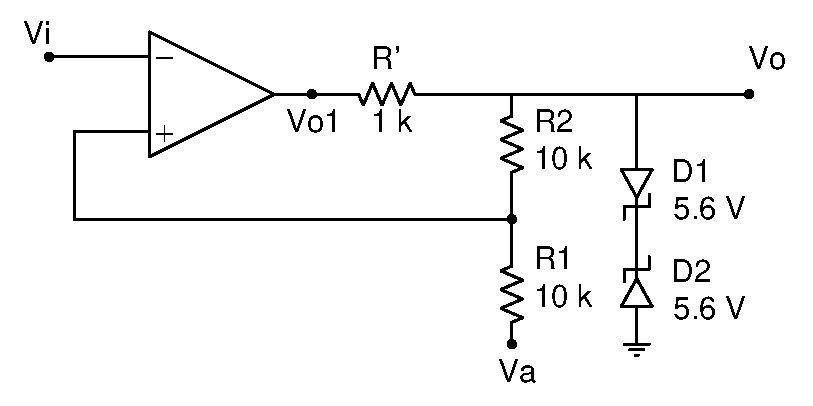
\includegraphics[scale=0.5]{schmitttriggerr.eps}
\caption{Schmitt Trigger}
\end{figure}

\subsection{Observations for Va = 0 V }
$V_{a}$=0 V,  $V_{in}$ = 12 V (pk-pk), 1 KHz 

\begin{figure}[h]
\centering
\begin{subfigure}{.5\textwidth}
  \centering
  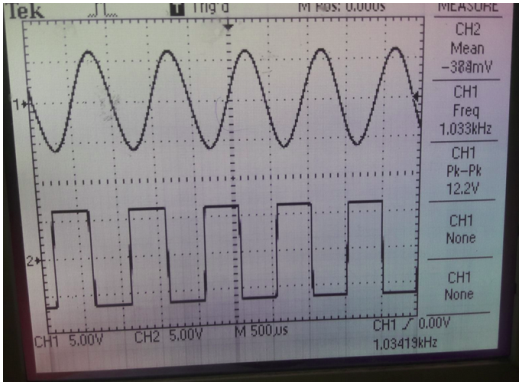
\includegraphics[width=.8\linewidth]{fig1.png}
  \caption{Input and Output Waveform}
  \label{fig:sub1}
\end{subfigure}%
\begin{subfigure}{.5\textwidth}
  \centering
  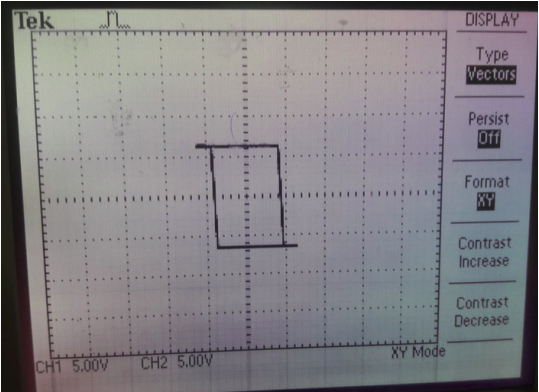
\includegraphics[width=.8\linewidth]{fig2.png}
  \caption{$V_{o}$ vs $V_{i}$ Plot}
  \end{subfigure}%
\\
\begin{subfigure}{.5\textwidth}
  \centering
  \includegraphics[width=.8\linewidth]{fig3.png}
  \caption{Delta showing the value of $V_{T}$}
  \label{fig:sub2}
\end{subfigure}
\caption{Waveforms for $V_{a}$=0 V}
\end{figure}



\subsubsection{Explanation}

\begin{equation}
    V_{T}=(\frac{R_{1}}{R_{1} + R_{2}})V_{O} + (\frac{R_{2}}{R_{1}+R_{2}})
 \end{equation}

for $V_{a}=0 V$ and $V_{O}=\pm5.6 V \pm0.7 = \pm 6.3 V$
\begin{equation}V_{T}=(\frac{10}{10 + 10})6.3 = 3.15 V
\end{equation}

Experimentally,delta comes out to be 3.92 V which is close to the theoretical value.


\begin{equation}
    A_{v}=\frac{V_{out}}{V_{1}-V_{2}} = \frac{R_{4}}{R_{3}}(1 + \frac{2R_{2}}{R_{1}})
\end{equation}
\subsection{Observations for Va = 3 V}
Va = 3 V, Vin = 12 V (pk-pk), 1 KHz

\begin{figure}[h]
\centering
\begin{subfigure}{.5\textwidth}
  \centering
  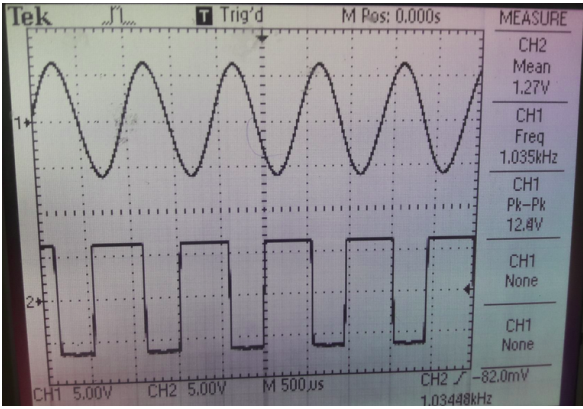
\includegraphics[width=.8\linewidth]{fi1.png}
  \caption{Input and Output Waveform}
  \label{fig:sub1}
\end{subfigure}%
\begin{subfigure}{.5\textwidth}
  \centering
  \includegraphics[width=.8\linewidth]{fi2.png}
  \caption{$V_{o}$ vs $V_{i}$ Plot}
  \label{fig:sub1}
\end{subfigure}%
\\
\begin{subfigure}{.5\textwidth}
  \centering
  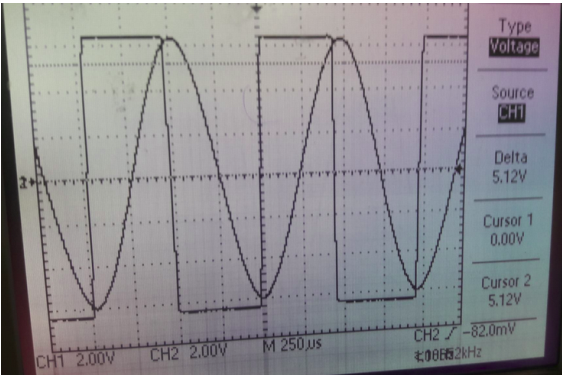
\includegraphics[width=.8\linewidth]{fi3.png}
  \caption{Cursor 2 showing the value of $V_{TH}$}
  \label{fig:sub2}
\end{subfigure}%
\begin{subfigure}{.5\textwidth}
  \centering
  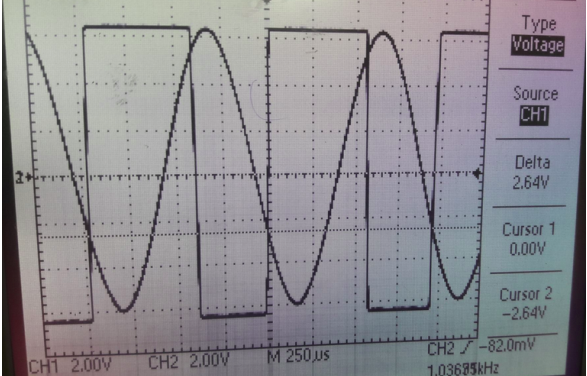
\includegraphics[width=.8\linewidth]{fi4.png}
  \caption{Cursor 2 showing the value of $V_{TL}$}
  \label{fig:sub2}
\end{subfigure}
\caption{Waveforms for $V_{a}$=3 V}
\end{figure}


\subsubsection{Explanation}

\begin{equation}
     V_{T}=(\frac{R_{1}}{R_{1} + R_{2}})V_{O} + (\frac{R_{2}}{R_{1}+R_{2}})V_{a}
\end{equation} 
\\for $V_{a}$= 0 V and $V_{O}$=\pm5.6 V \pm0.7 = \pm 6.3 V

So,we get $V_{TH}$=4.6 V and $V_{TL}$=-1.65 V
\\The experimental values are very close to the theoretically calculated values.
\newpage
\section{Astable Multivibrator}

Output waveform when potentiometer is close to 10 k\si{\ohm}



\begin{figure}[h]
  % will center the figure.
  \centering
  % include graphics (can include eps, jpg, pdf ...)
  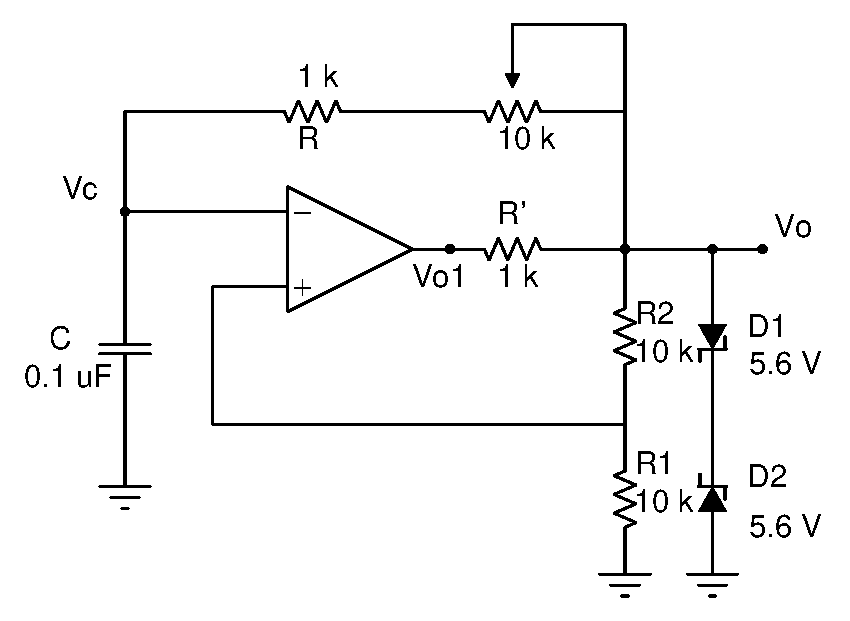
\includegraphics[scale=0.6]{astaable2.eps}  % change scale factor to re-size the image.
  % give a caption.
  \caption{Astable Multivibrator}
\end{figure}

\subsection{Observations}
\begin{figure}[h]
  % will center the figure.
  \centering
  % include graphics (can include eps, jpg, pdf ...)
  \includegraphics[scale=0.4]{wavef.png}  % change scale factor to re-size the image.
  % give a caption.
  \caption{Output waveform when resistance of the potentiometer is close to 10 k\si{\ohm}}
\end{figure}

\newpage
%
% Tables.
%
\begin{table}[h]
\centering  % table will be centered.
\begin{tabular}{|c | c| c|} % 3 columns, with text centered in each column, 
			 %  the | specifies that there will be a line separating the
			 %  adjacent columns.
\hline  % horizontal line spanning the columns.
Potentiometer Value(k\si{\ohm}) & Theoretical Value(Hz) & Experimental Frequency(Hz) \\  % table entry 1, separated by &, ended by \\
\hline  % horizontal line spanning the columns.
10    & 413 & 563.1 \\  % table entry 2, separated by &, ended by \\
0    & 4.55 k & 5.14 k \\  % ...
\hline	% horizontal line.
\end{tabular}
\caption{Observation table for Astable Multivibrator}
\end{table}
\\
\subsection{Explanation}
When potentiometer value is close to 0 \si{\ohm}, the frequency is very high, thus, the pulse width
reduces and the capacitor doesn't get time to charge. Hence we see a distortion in the
waveform.
\end{document}
